Figure \ref{area_rep} shows the variation of the area of both half adder and full adder as the gate width increases by 20\% for each node. It is clear that the area is linearly dependent with the width of the transistor.
\begin{figure}[h]
	\caption{MATLAB area plot}
	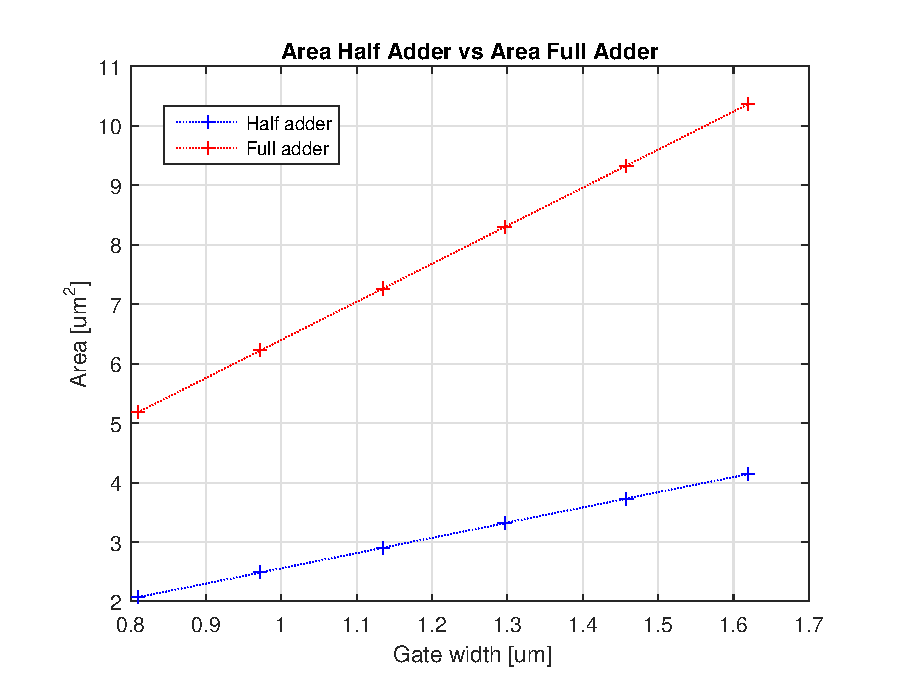
\includegraphics{img/area_rep}
	\centering
	\label{area_rep}
\end{figure}

\newpage
Figure \ref{delay_rep} shows the dependency between the delay of both half adder and full adder to the gate width. The plot shows an asintotic behavior, explained by the fact that the NAND capacitance is not affected by the variation of the gate width (almost remaining constant), while instead having the driving current of the NAND gate linearly increasing. Since the delay is inversely proportional to the driving current, this explains the obtained results.
\begin{figure}[h]
	\caption{MATLAB delay plot}
	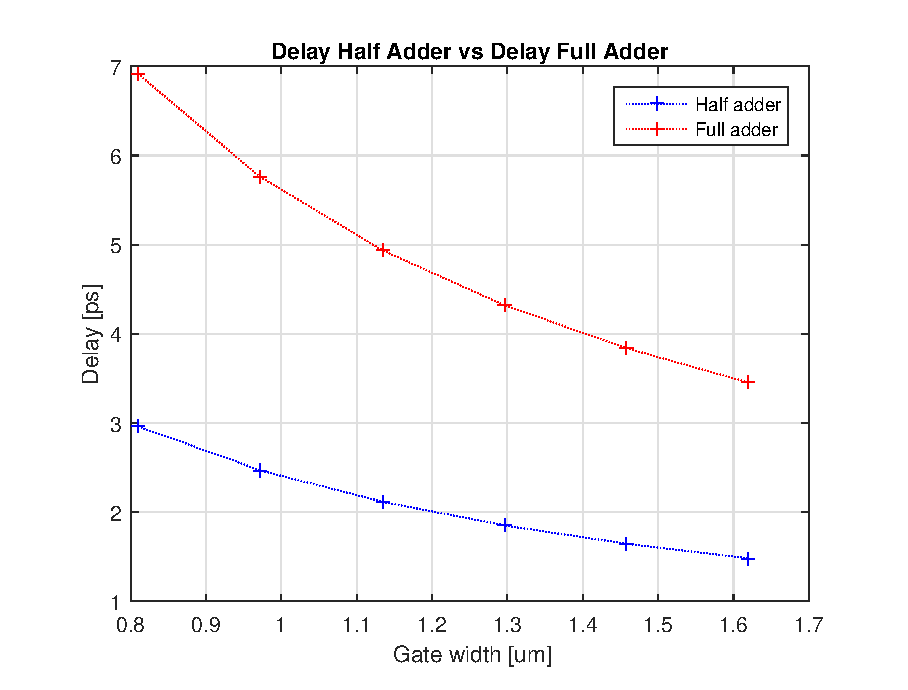
\includegraphics{img/delay_rep}
	\centering
	\label{delay_rep}
\end{figure}

\newpage
Figure \ref{freq_rep} shows the dependency between frequency of half adder and full adder to the gate width. Since it is the inverse of the critical path, the behavior is simply linear.
\begin{figure}[h]
	\caption{MATLAB freq plot}
	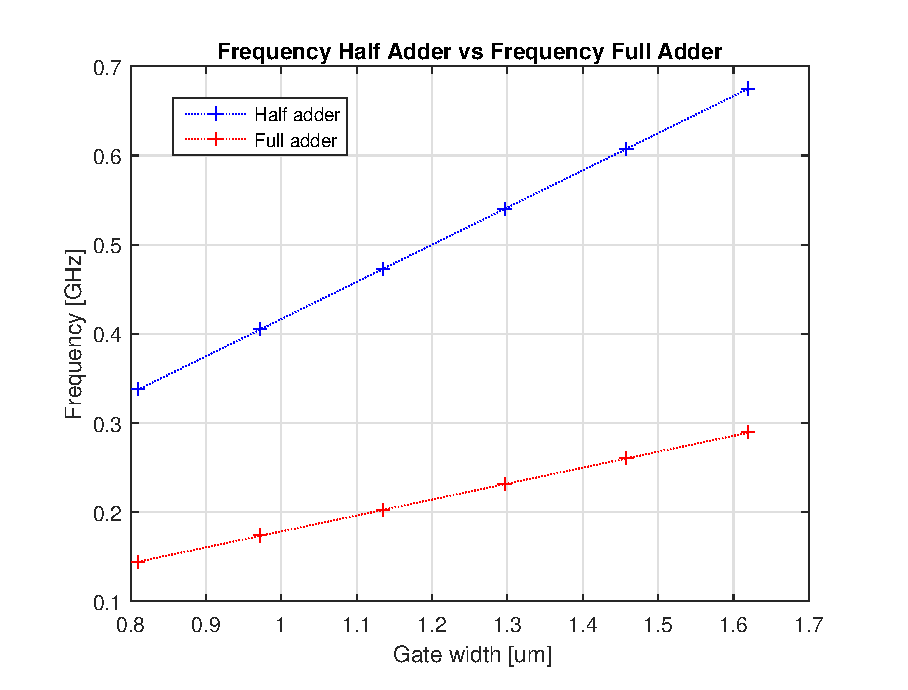
\includegraphics{img/freq_rep}
	\centering
	\label{freq_rep}
\end{figure}

\newpage
Figure \ref{power_rep} shows the dependency of the power consumption of both half adder and full adder in respect to the gate width, considering a fixed switching activity. The dynamic power is linearly dependent to the frequency (which has a linear tendence) and to the NAND capacity. Therefore, the result will be a linear plot as well.
\begin{figure}[h]
	\caption{MATLAB power plot}
	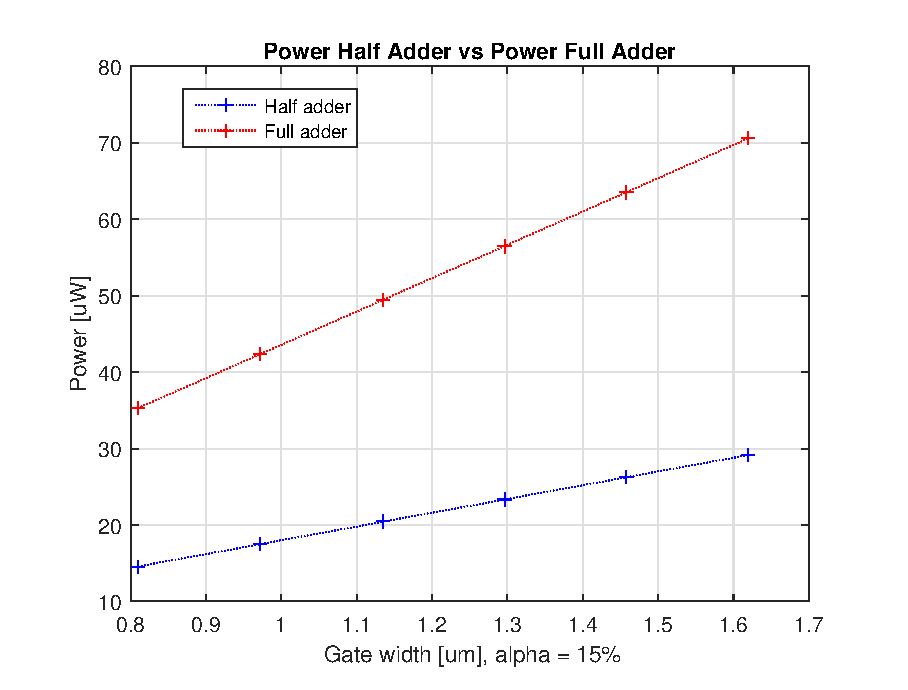
\includegraphics{img/power_rep}
	\centering
	\label{power_rep}
\end{figure}

\newpage
Figure \ref{power_rep_swt_act} shows the dependency of the variation of the switching activity of the system to the overall power consumption, considering a fixed gate width. The trend of the power consumption is still linear, but higher $\alpha$ show an higher power consumption in respecto to higher values of the gate width.
\begin{figure}[h]
	\caption{MATLAB power plot}
	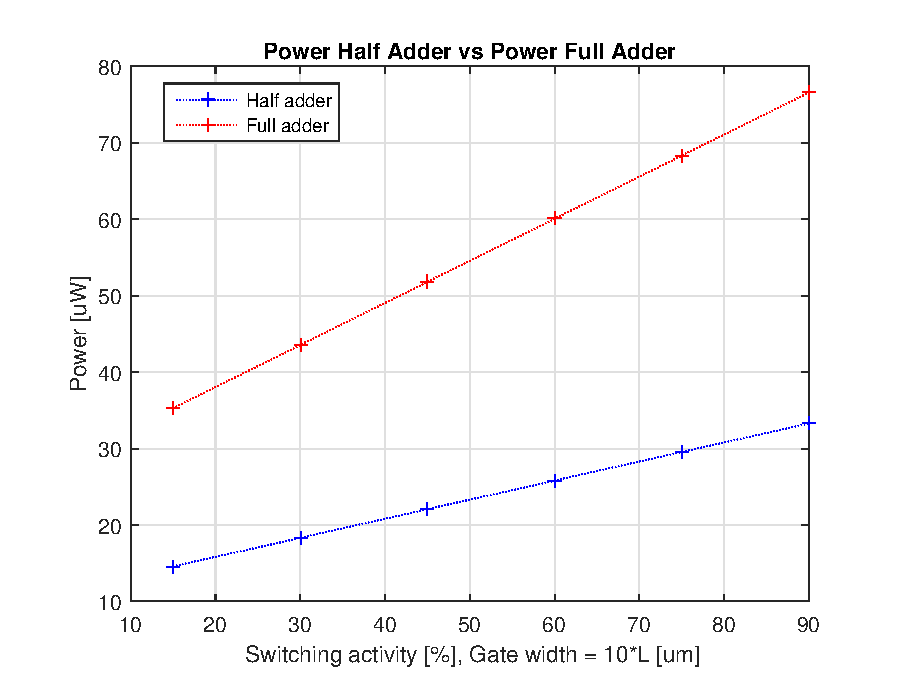
\includegraphics{img/power_rep_swt_act}
	\centering
	\label{power_rep_swt_act}
\end{figure}